\section{Einschr"ankung des Zielgebiets}
H"aufig kommt es vor, dass das Optimum innerhalb eines bestimmten
Zielgebiets gesucht wird. Daher m"ussen Mittel gefunden werden die
verhindern, dass die Partikel einen Definitionsbereich verlassen und
nicht mehr zur L"osungsfindung beitragen. Die einfachste M"oglichkeit
ist, den Fitnesswert von Partikeln ausserhalb des Definitionsgebiets auf
einen schlechten Wert zu setzen. Trotzdem ben"otigt das Partikel meist
mehrere Iterationen um zur"uck in das Definitionsgebiet zu finden.

Eine verbreitete L"osung ist, das Partikel auf die Grenze des Bereichs und
die Geschwindigkeit auf 0 zu setzen. Dieser Ansatz hat sich gegen"uber
dem ``Abprallen'' an der Bereichsgrenze durchgesetzt, weil so Optima am
Rand des Zielgebiets besser erkannt werden k"onnen.

\section{Maximale Geschwindigkeit}
Ein bekanntes Problem der Partikelschwarm-Optimierung ist, dass die
Geschwindigkeit eines Partikels schnell sehr hohe Werte annimmt. Das
kann so weit gehen, dass ganze Teilgebiete durch die hohe Geschwindigkeit
"ubersprungen werden. Die L"osung f"ur dieses Problem ist die Einf"uhrung
einer maximalen Geschwindigkeit, \textit{velocity clamping} genannt. Die
Geschwindigkeit wird also nach folgender Formel berechnet:
\begin{equation}
	v_{ij}(t+1) = 
	\begin{cases}
		v_{ij}(t+1) & \text{falls $|v_{ij}(t+1)| < V_{max,j}$}\\
		V_{max,j} & \text{falls $|v_{ij}(t+1)| \geq V_{max,j}$}
	\end{cases}
	\label{eqn-max-velocity}
\end{equation}
Diese Erweiterung sorgt daf"ur, dass ein gr"osserer Bereich des Suchraums
erforscht wird. Der optimale Wert f"ur $V_{max,j}$ ist vom Problem
abh"angig und kann nicht generell bestimmt werden. \\

Wie die Gleichung \ref{eqn-max-velocity} zeigt, wird die Geschwindigkeit
f"ur jede Dimension einzeln beschr"ankt. Damit ergibt sich graphisch
die Situation von Abbildung~\ref{fig-max-velocity}.

\begin{figure}[htbp]
	\centering
	\documentclass{standalone}

\usepackage{tikz}
\usetikzlibrary{arrows,decorations.pathmorphing,positioning,fit,petri}
\usetikzlibrary{calc,intersections,through,backgrounds,graphs}
\usetikzlibrary{patterns,decorations.pathreplacing}

\begin{document}

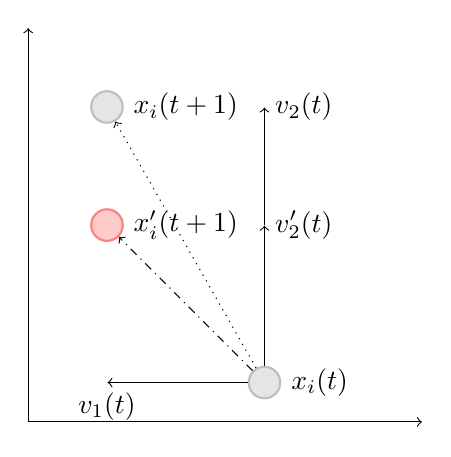
\begin{tikzpicture}
	% Styles
	[
	point/.style={circle,inner sep=0pt,minimum size=0mm},
	vpoint/.style={circle,draw=gray!50,fill=gray!20,thick, inner sep=0pt,minimum size=4mm},
	endpoint/.style={circle,draw=red!50,fill=red!20,thick, inner sep=0pt,minimum size=4mm},
	]
                      
	% Axis
	\draw[->] (0,0) -- (5,0);
  	\draw[->] (0,0) -- (0,5);

	% Nodes
	\node at (3,0.5)	(xi1)	[vpoint]	{};
	\node at (1,4)	(xi2) [vpoint] {};
	\node at (1,2.5)	(xi3) [endpoint] {};
	\node at (3,2.5) 	(v2) [point] {};
	\node at (3,4)	(v22) [point] {};
	\node at (1,0.5)	(v1) [point] {};

	% Arrows	
	\draw[->] (xi1) -- (v2);
	\draw[->] (v2) -- (v22);
	\draw[->] (xi1) -- (v1);
	\draw[->,dotted] (xi1) -- (xi2);
	\draw[->,dashdotted] (xi1) -- (xi3);

	% Text
	\node at (3.7,0.5) {$x_i(t)$};
	\node at (2,4) {$x_i(t+1)$};
	\node at (2,2.5) {$x_i'(t+1)$};
	\node at (3.5,4) {$v_2(t)$};
	\node at (3.5,2.5) {$v_2'(t)$};
	\node at (1,0.2) {$v_1(t)$};
\end{tikzpicture}

\end{document}
	\caption{Einf"uhren einer maximalen Geschwindigkeit}
	\label{fig-max-velocity}
\end{figure}

Die Geschwindigkeit $v_2(t)$ ist hier gr"osser als die maximale
Geschwindigkeit $V_{max}$, weshalb sie auf $v'_2$ reduziert wird. Die
Geschwindigkeit $v_1$ wird jedoch nicht ver"andert. \\

Diese Geschwindigkeitsbegrenzung f"uhrt jedoch zu Problemen, wenn alle
Geschwindigkeiten h"oher als die Begrenzung sind: Die Teilchen suchen
dann nur an den Kanten eines $n$-dimensionalen Hyperw"urfels. Als
Gegenmassnahme kann gem"ass \cite{schutte-sizing} $V_{max,j}$ dynamisch
angepasst werden, wenn sich die global beste Position gbest "uber eine
Anzahl $\tau$ Iterationen nicht verbessert:
\begin{equation}
	V_{max,j} = 
	\begin{cases}
		\beta V_{max,j} & \text{falls $f(\hat{y}(t)) \geq f(\hat{y}(t-t')) 
			 \qquad  \forall \: t' = \{ 1, \dots, \tau \}$} \\
		V_{max,j} & \text{onst}
	\end{cases}
\end{equation}
mit $0 < \beta < 1$.

Um eine h"ohere Genauigkeit zu erreichen kann die maximale Geschwindigkeit
im Verlauf der Zeit exponentiell verringert werden:
\begin{equation}
	V_{max,j}(t+1) = \left(1-\left(\frac{t}{T}\right)^{\alpha}\right) V_{max,j}(t)
\end{equation}
$T$ ist hier die maximale Anzahl Iterationen. Der Faktor $\alpha$
ist abh"angig von der Problemstellung und es existieren gem"ass
\cite{Han-Modification} keine mathematischen Hintergr"unde zur exakten
Bestimmung.
